\chapter{PRESENTACI�N Y AN�LISIS DE RESULTADOS}
\section{Selecci\'on del movimiento de cada equipo deportivo} \label{res:idMov}
\begin{figure}[H]
	\caption{Formulario de movimiento de tenis de mesa}
	\label{fig:frmMovTen}
	\centering
	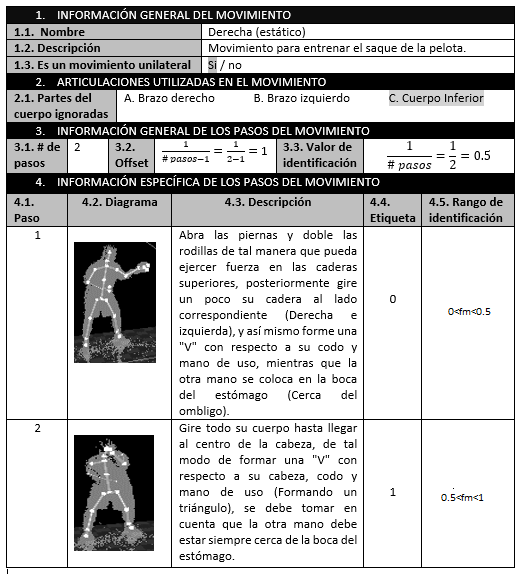
\includegraphics[width=430px,height=360px]{graphics/resultados/movimientoTenis.PNG} \\
	\textbf{Fuente:} Elaborado por el autor de tesis en base a las observaciones del trabajo de campo
\end{figure}
\begin{figure}[H]
	\caption{Formulario de movimiento de animaci\'on}
	\label{fig:frmMovCheer}
	\centering
	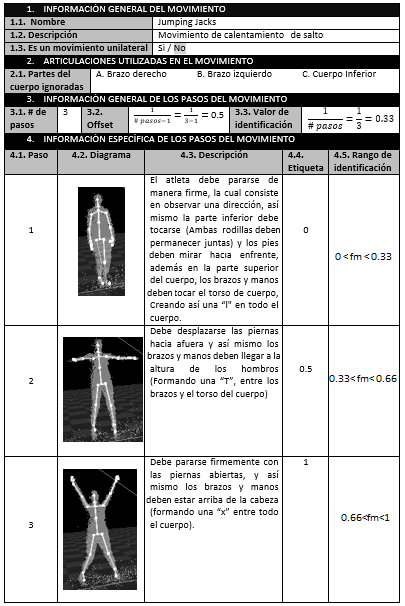
\includegraphics[width=445px,height=600px]{graphics/resultados/movimientoCheerleader.PNG} \\
	\textbf{Fuente:} Elaborado por el autor de tesis en base a las observaciones del trabajo de campo
\end{figure}
\begin{figure}[H]
	\caption{Formulario de movimiento taekwondo}
	\label{fig:frmWhiteMov}
	\centering
	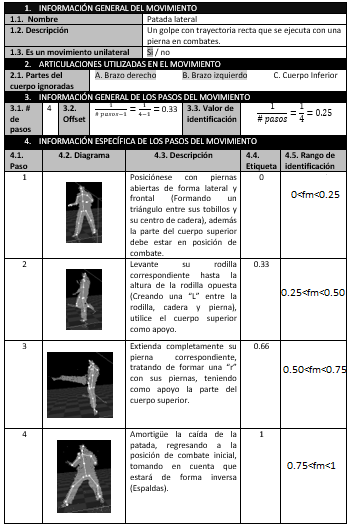
\includegraphics[width=445px,height=600px]{graphics/resultados/movimientoTaekwondo.PNG} \\
	\textbf{Fuente:} Elaborado por el autor de tesis en base a las observaciones del trabajo de campo
\end{figure}
\section{Creaci\'on de rutina del movimiento de cada equipo deportivo} \label{res:idMov}
\begin{figure}[H]
	\caption{Formulario de rutina de animaci\'on}
	\label{fig:frmRoutCher}
	\centering
	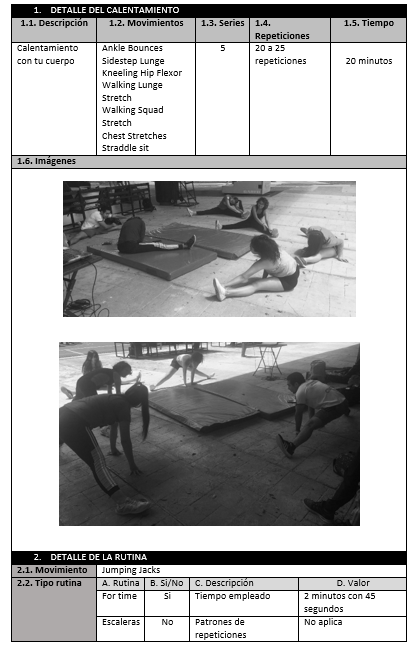
\includegraphics[width=445px,height=550px]{graphics/resultados/rutina-cheerleaders.PNG} \\
	\textbf{Fuente:} Elaborado por el autor de tesis en base a las observaciones del trabajo de campo
\end{figure}
\begin{figure}[H]
	\caption{Formulario de rutina de tenis de mesa}
	\label{fig:frmRoutTen}
	\centering
	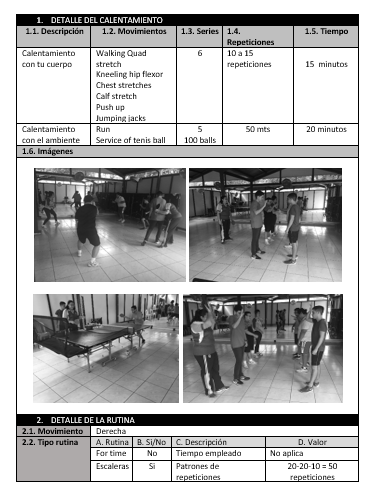
\includegraphics[width=445px,height=600px]{graphics/resultados/rutina-tennis.PNG} \\
	\textbf{Fuente:} Elaborado por el autor de tesis en base a las observaciones del trabajo de campo
\end{figure}
\begin{figure}[H]
	\caption{Formulario de rutina de taekwondo}
	\label{fig:frmRoutTaek}
	\centering
	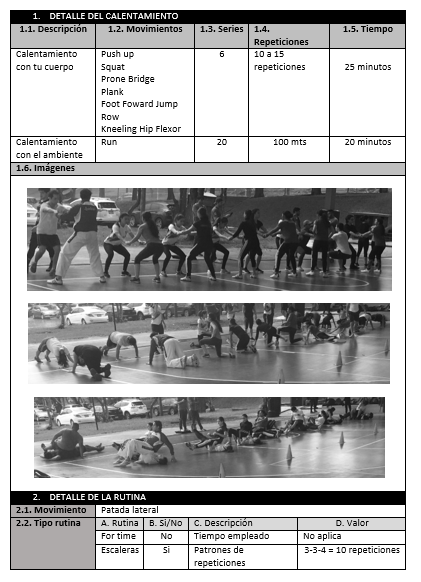
\includegraphics[width=445px,height=600px]{graphics/resultados/rutina-taekwondo.PNG} \\
	\textbf{Fuente:} Elaborado por el autor de tesis en base a las observaciones del trabajo de campo
\end{figure}
\section{Distancias de profundidad recomendadas entre el atleta y el sensor} \label{res:idMov}
\begin{table}[H]
\begin{center}
\caption{Distancias de profundidad con respecto a la cadera central del atleta, tomada a una altura del Kinect de 0.70 mts (Medida a partir del suelo)}
\label{tab:depthCalculation}
\begin{tabular}{lllll}
\hline
\multicolumn{3}{|c|}{Caracter\'isticas generales} & \multicolumn{2}{l|}{\begin{tabular}[c]{@{}l@{}}Distancia de profundidad\\ recomendada entre el \\ usuario y el sensor\end{tabular}} \\ \hline
\multicolumn{1}{|l|}{Deporte} & \multicolumn{1}{l|}{\begin{tabular}[c]{@{}l@{}}Altura promedio\\ (Metros)\end{tabular}} & \multicolumn{1}{l|}{\begin{tabular}[c]{@{}l@{}}Desviaci\'on est\'andar\\ de la altura (metros)\end{tabular}} & \multicolumn{1}{l|}{\begin{tabular}[c]{@{}l@{}}M\'inima\\ (Metros)\end{tabular}} & \multicolumn{1}{l|}{\begin{tabular}[c]{@{}l@{}}M\'axima\\ (Metros)\end{tabular}} \\ \hline
\multicolumn{1}{|l|}{Tenis de mesa} & \multicolumn{1}{l|}{1.302435} & \multicolumn{1}{l|}{0.088683} & \multicolumn{1}{l|}{3.505103} & \multicolumn{1}{l|}{3.990376} \\ \hline
\multicolumn{1}{|l|}{Animaci\'on} & \multicolumn{1}{l|}{1.342471} & \multicolumn{1}{l|}{0.059301} & \multicolumn{1}{l|}{2.763813} & \multicolumn{1}{l|}{3.411942} \\ \hline
\multicolumn{1}{|l|}{Taekwondo} & \multicolumn{1}{l|}{1.373372} & \multicolumn{1}{l|}{0.098490} & \multicolumn{1}{l|}{2.556640} & \multicolumn{1}{l|}{3.869427} \\ \hline
\multicolumn{5}{l}{\textbf{Fuente:} Instrumento \ref{ins:UI:wpf}.\ref{ins:UI:wpf:depth} utilizado en los atletas de construcci\'on y pruebas (ver secci\'on \ref{sj:1t})}
\end{tabular}
\end{center}
\end{table}
\section{Muestras de fotogramas del movimiento} \label{res:fotogramas}
\begin{figure}[H]
	\caption{Fotogramas de 6 sujetos del equipo de tenis de mesa}
	\label{fig:fotogramaTenis}
	\centering
	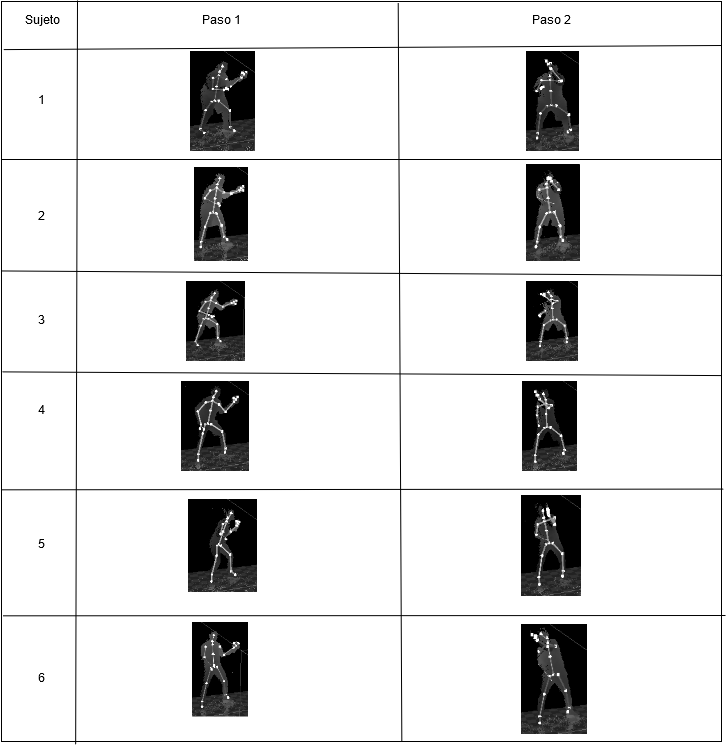
\includegraphics[width=430px,height=300px]{graphics/resultados/SETenisDeMesa.PNG} \\
	\textbf{Fuente:} Recuperado por los v\'ideos de trabajo de campo (ver instrumento \ref{ins:KinectStudio})
\end{figure}
\begin{figure}[H]
	\caption{Fotogramas de 7 sujetos del equipo de animaci\'on}
	\label{fig:fotogramaCheerleader}
	\centering
	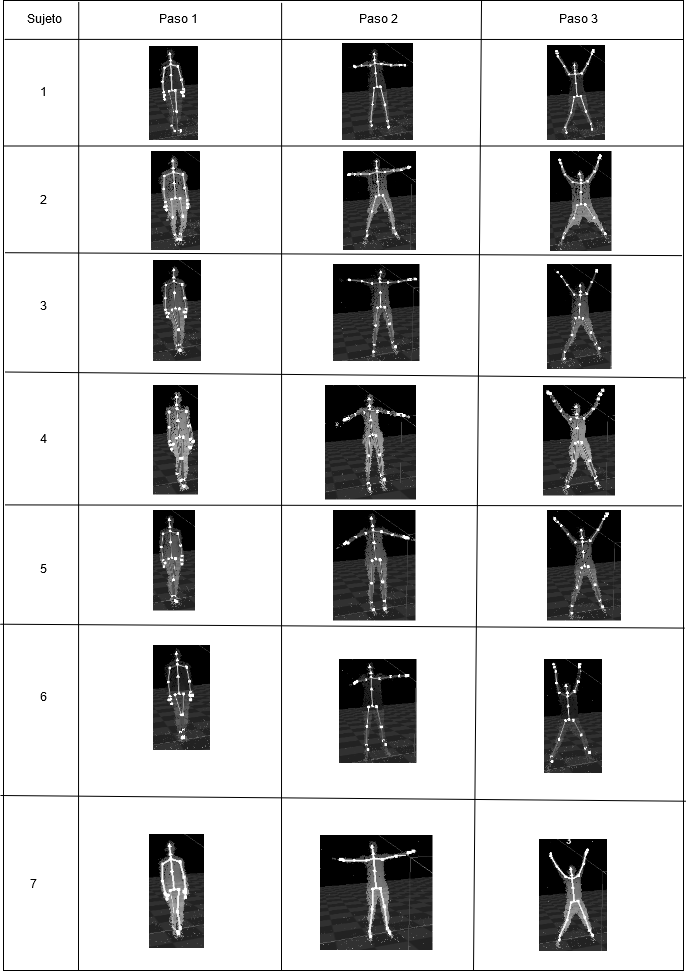
\includegraphics[width=445px,height=600px]{graphics/resultados/SECheerleaders.PNG} \\
	\textbf{Fuente:} Recuperado por los v\'ideos de trabajo de campo (ver instrumento \ref{ins:KinectStudio})
\end{figure}
\begin{figure}[H]
	\caption{Fotogramas de 7 sujetos del equipo de taekwondo}
	\label{fig:fotogramaTaekwondo}
	\centering
	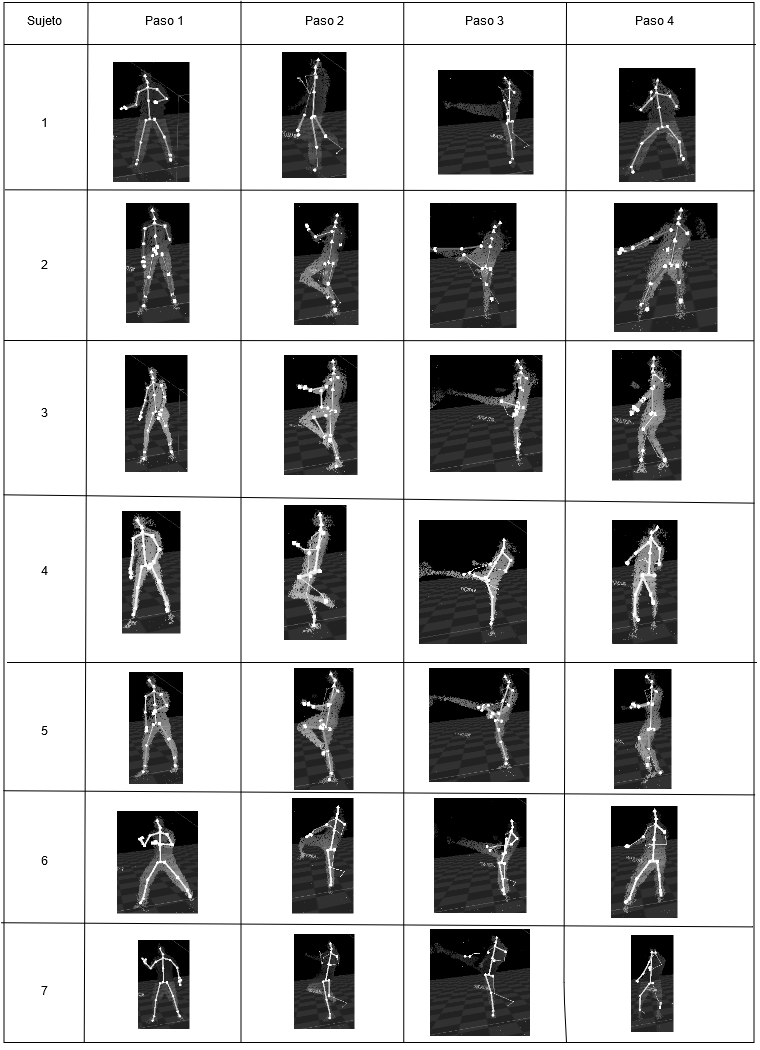
\includegraphics[width=445px,height=600px]{graphics/resultados/SETaekwondo.PNG} \\
	\textbf{Fuente:} Recuperado por los v\'ideos de trabajo de campo (ver instrumento \ref{ins:KinectStudio})
\end{figure}
\begin{landscape}
\section{Razones de fallo del seguimiento de esqueleto}
\begin{figure}[H]
	\caption{diagrama de Ishikawa sobre el fallo del seguimiento de esqueleto}
	\label{fig:ishikawa}
	\centering
	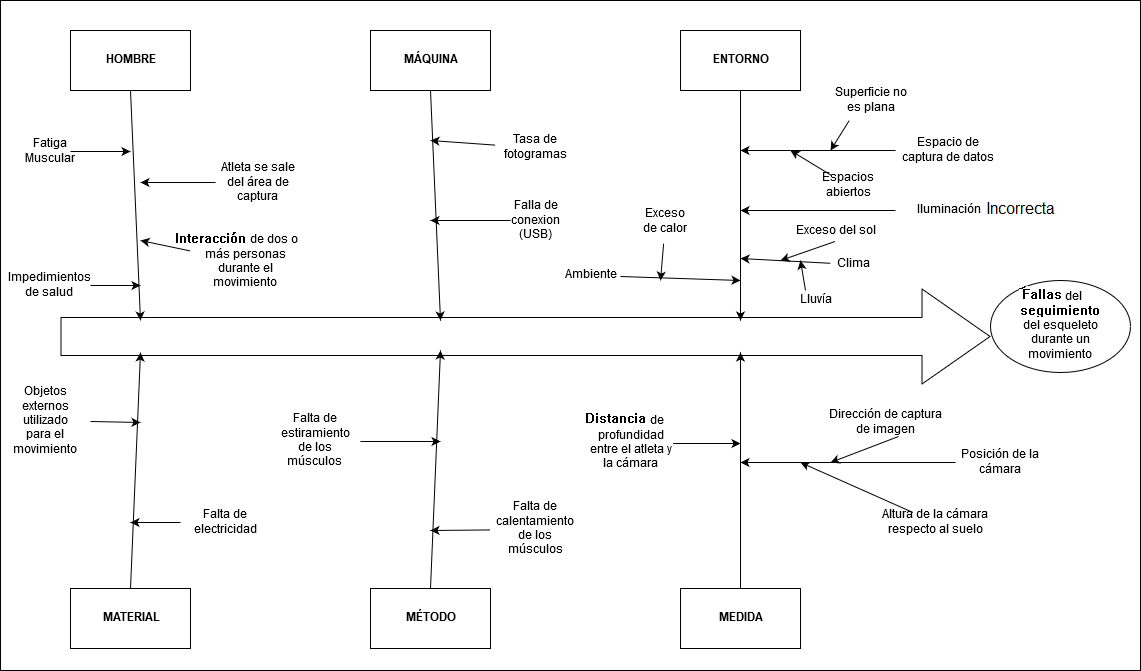
\includegraphics[width=610px,height=380px]{graphics/resultados/Ishi-SeguimientoDeEsqueleto.PNG} \\
	\textbf{Fuente:} Realizado en base a las observaciones de trabajo de campo.
\end{figure}
\end{landscape}
\section{Proceso de etiquetaci\'on de un movimiento}
\begin{figure}[H]
	\caption{Etiquetaci\'on de fotogramas del equipo de tenis de mesa}
	\label{fig:etiquetaTenis}
	\centering
	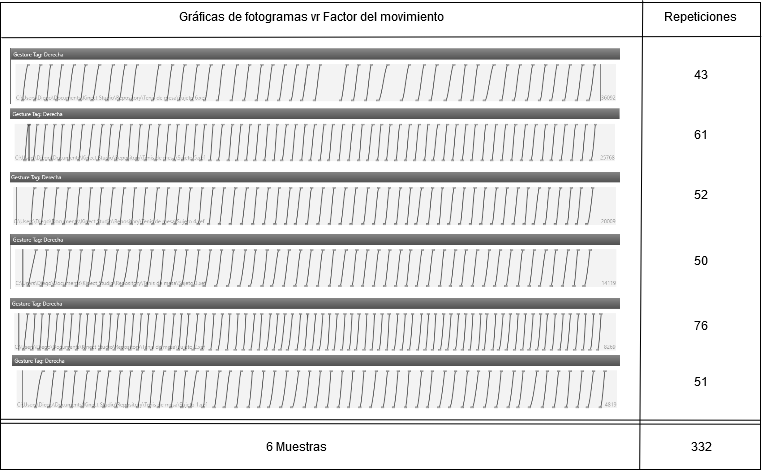
\includegraphics[width=445px,height=260px]{graphics/resultados/GraSegTenisDeMesa.PNG} \\
	\textbf{Fuente:} Recuperado por los v\'ideos etiquetados del trabajo de campo (ver instrumento \ref{ins:VisualGestureBuilder})
\end{figure}
\begin{figure}[H]
	\caption{Etiquetaci\'on de fotogramas del equipo de animaci\'on}
	\label{fig:etiquetaCheerleader}
	\centering
	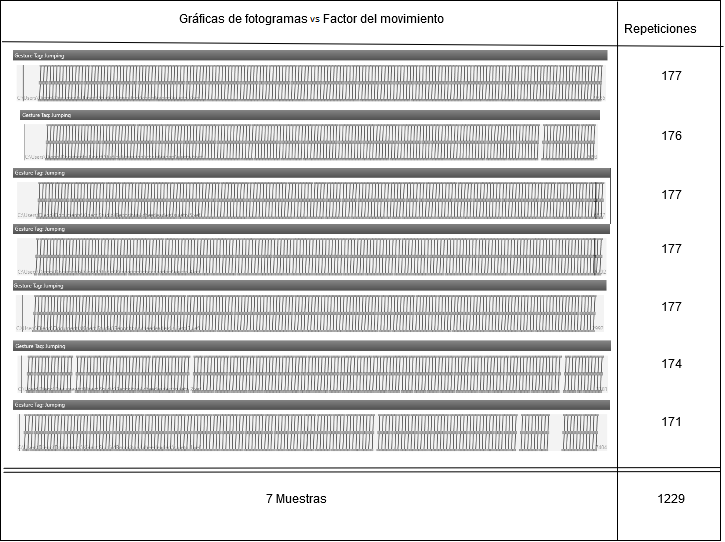
\includegraphics[width=445px,height=260px]{graphics/resultados/GraSegCheerleaders.PNG} \\
	\textbf{Fuente:} Recuperado por los v\'ideos etiquetados del trabajo de campo (ver instrumento \ref{ins:VisualGestureBuilder})
\end{figure}
\begin{figure}[H]
	\caption{Etiquetaci\'on de fotogramas del equipo de taekwondo}
	\label{fig:etiquetaTaekwondo}
	\centering
	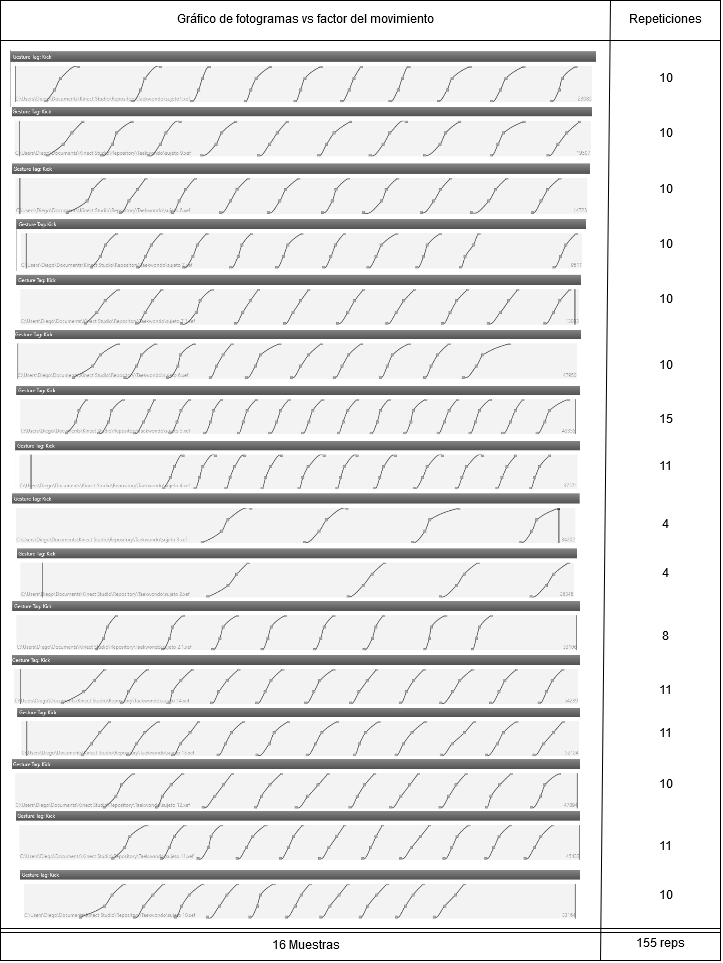
\includegraphics[width=445px,height=580px]{graphics/resultados/GraSegTaekwondo.PNG} \\
	\textbf{Fuente:} Recuperado por los v\'ideos etiquetados del trabajo de campo (ver instrumento \ref{ins:VisualGestureBuilder})
\end{figure}
\section{Selecci\'on y pruebas del modelo} \label{res:chooseModel}
\begin{table}[H]
\begin{center}
\caption{Modelos y pruebas del equipo de Taekwondo}
\label{tab:chooseTaekwondo}
\begin{tabular}{cccc}
\hline
\multicolumn{4}{|c|}{1. Datos de los errores de los modelos} \\ \hline
\multicolumn{1}{|c|}{\textbf{Modelo}} & \multicolumn{1}{c|}{\textbf{EMP}} & \multicolumn{1}{c|}{\textbf{DAM}} & \multicolumn{1}{c|}{\textbf{RECM}} \\ \hline
\multicolumn{1}{|c|}{1} & \multicolumn{1}{c|}{-0,03543} & \multicolumn{1}{c|}{0,301911} & \multicolumn{1}{c|}{0,374544078} \\ \hline
\multicolumn{1}{|c|}{2} & \multicolumn{1}{c|}{0,050888} & \multicolumn{1}{c|}{0,297433} & \multicolumn{1}{c|}{0,393153} \\ \hline
\multicolumn{1}{|c|}{3} & \multicolumn{1}{c|}{0,200827} & \multicolumn{1}{c|}{0,214594} & \multicolumn{1}{c|}{0,191583} \\ \hline
\multicolumn{1}{|c|}{\textbf{Promedio}} & \multicolumn{1}{c|}{0,072095} & \multicolumn{1}{c|}{0,271313} & \multicolumn{1}{c|}{0,31976} \\ \hline
\multicolumn{1}{l}{} & \multicolumn{1}{l}{} & \multicolumn{1}{l}{} & \multicolumn{1}{l}{} \\ \hline
\multicolumn{4}{|c|}{2. Detalle del modelo} \\ \hline
\multicolumn{3}{|c|}{\textbf{Mejor modelo}} & \multicolumn{1}{c|}{3} \\ \hline
\multicolumn{3}{|c|}{\textbf{Aprueba o rechaza el modelo}} & \multicolumn{1}{c|}{\begin{tabular}[c]{@{}c@{}}Rechaza\\ 0,31976  \textgreater{}= 0.25\end{tabular}} \\ \hline
\multicolumn{3}{|c|}{\textbf{Recognition}} & \multicolumn{1}{c|}{1,27904} \\ \hline
\multicolumn{4}{l}{\textbf{Fuente:} c\'alculo de intervalos de confianza (ver f\'ormula \ref{frm:rangoConfiabilidad})}
\end{tabular}
\end{center}
\end{table}
\begin{table}[H]
\begin{center}
\caption{Modelos y pruebas del equipo de tenis de mesa }
\label{tab:chooseModelTenis}
\begin{tabular}{cccc}
\hline
\multicolumn{4}{|c|}{1. Datos de los errores de los modelos} \\ \hline
\multicolumn{1}{|c|}{\textbf{Modelo}} & \multicolumn{1}{c|}{\textbf{EMP}} & \multicolumn{1}{c|}{\textbf{DAM}} & \multicolumn{1}{c|}{\textbf{RECM}} \\ \hline
\multicolumn{1}{|c|}{1} & \multicolumn{1}{c|}{0,175144} & \multicolumn{1}{c|}{0,217553} & \multicolumn{1}{c|}{0,236069} \\ \hline
\multicolumn{1}{|c|}{2} & \multicolumn{1}{c|}{0,022738} & \multicolumn{1}{c|}{0,113367} & \multicolumn{1}{c|}{0,140393} \\ \hline
\multicolumn{1}{|c|}{3} & \multicolumn{1}{c|}{0,139513} & \multicolumn{1}{c|}{0,260699} & \multicolumn{1}{c|}{0,342375} \\ \hline
\multicolumn{1}{|c|}{\textbf{Promedio}} & \multicolumn{1}{c|}{0,112465} & \multicolumn{1}{c|}{0,197206} & \multicolumn{1}{c|}{0,239612} \\ \hline
\multicolumn{1}{l}{} & \multicolumn{1}{l}{} & \multicolumn{1}{l}{} & \multicolumn{1}{l}{} \\ \hline
\multicolumn{4}{|c|}{2. Detalle del modelo} \\ \hline
\multicolumn{3}{|c|}{\textbf{Mejor modelo}} & \multicolumn{1}{c|}{2} \\ \hline
\multicolumn{3}{|c|}{\textbf{Aprueba o rechaza el modelo}} & \multicolumn{1}{c|}{\begin{tabular}[c]{@{}c@{}}Aprueba\\ 0,239612 \textless 0.5\end{tabular}} \\ \hline
\multicolumn{3}{|c|}{\textbf{Recognition}} & \multicolumn{1}{c|}{0,479225} \\ \hline
\multicolumn{1}{l}{} & \multicolumn{1}{l}{} & \multicolumn{1}{l}{} & \multicolumn{1}{l}{} \\ \hline
\multicolumn{4}{|c|}{3. Detalle del paso del movimiento} \\ \hline
\multicolumn{2}{|c|}{\textbf{Detallle}} & \multicolumn{2}{c|}{\textbf{Intervalo de confianza}} \\ \hline
\multicolumn{1}{|c|}{Paso} & \multicolumn{1}{c|}{Etiqueta} & \multicolumn{1}{c|}{Inferior} & \multicolumn{1}{c|}{Superior} \\ \hline
\multicolumn{1}{|c|}{1} & \multicolumn{1}{c|}{0} & \multicolumn{1}{c|}{0} & \multicolumn{1}{c|}{0,239612} \\ \hline
\multicolumn{1}{|c|}{2} & \multicolumn{1}{c|}{1} & \multicolumn{1}{c|}{0,760388} & \multicolumn{1}{c|}{1} \\ \hline
\multicolumn{4}{l}{\textbf{Fuente:} c\'alculo de intervalos de confianza (ver f\'ormula \ref{frm:rangoConfiabilidad})}
\end{tabular}
\end{center}
\end{table}
\begin{table}[H]
\begin{center}
\caption{Modelos y pruebas del equipo de animaci\'on}
\label{tab:chooseCheerleader}
\begin{tabular}{cccc}
\hline
\multicolumn{4}{|c|}{1. Datos de los errores de los modelos} \\ \hline
\multicolumn{1}{|c|}{\textbf{Modelo}} & \multicolumn{1}{c|}{\textbf{EMP}} & \multicolumn{1}{c|}{\textbf{DAM}} & \multicolumn{1}{c|}{\textbf{RECM}} \\ \hline
\multicolumn{1}{|c|}{1} & \multicolumn{1}{c|}{0,02323} & \multicolumn{1}{c|}{0,038519} & \multicolumn{1}{c|}{0,046957} \\ \hline
\multicolumn{1}{|c|}{2} & \multicolumn{1}{c|}{0,080008} & \multicolumn{1}{c|}{0,083864} & \multicolumn{1}{c|}{0,076391} \\ \hline
\multicolumn{1}{|c|}{3} & \multicolumn{1}{c|}{0,032244} & \multicolumn{1}{c|}{0,04105} & \multicolumn{1}{c|}{0,045347} \\ \hline
\multicolumn{1}{|c|}{\textbf{Promedio}} & \multicolumn{1}{c|}{0,045161} & \multicolumn{1}{c|}{0,054478} & \multicolumn{1}{c|}{0,056232} \\ \hline
\multicolumn{1}{l}{} & \multicolumn{1}{l}{} & \multicolumn{1}{l}{} & \multicolumn{1}{l}{} \\ \hline
\multicolumn{4}{|c|}{2. Detalle del modelo} \\ \hline
\multicolumn{3}{|c|}{\textbf{Mejor modelo}} & \multicolumn{1}{c|}{3} \\ \hline
\multicolumn{3}{|c|}{\textbf{Aprueba o rechaza el modelo}} & \multicolumn{1}{c|}{\begin{tabular}[c]{@{}c@{}}Aprueba\\ 0,056232 \textless 0.33\end{tabular}} \\ \hline
\multicolumn{3}{|c|}{\textbf{Recognition}} & \multicolumn{1}{c|}{0,168695} \\ \hline
\multicolumn{1}{l}{} & \multicolumn{1}{l}{} & \multicolumn{1}{l}{} & \multicolumn{1}{l}{} \\ \hline
\multicolumn{4}{|c|}{3. Detalle del paso del movimiento} \\ \hline
\multicolumn{2}{|c|}{\textbf{Detallle}} & \multicolumn{2}{c|}{\textbf{Intervalo de confianza}} \\ \hline
\multicolumn{1}{|c|}{Paso} & \multicolumn{1}{c|}{Etiqueta} & \multicolumn{1}{c|}{Inferior} & \multicolumn{1}{c|}{Superior} \\ \hline
\multicolumn{1}{|c|}{1} & \multicolumn{1}{c|}{0} & \multicolumn{1}{c|}{0} & \multicolumn{1}{c|}{0,056232} \\ \hline
\multicolumn{1}{|c|}{2} & \multicolumn{1}{c|}{0.5} & \multicolumn{1}{c|}{0,471884} & \multicolumn{1}{c|}{0,528116} \\ \hline
\multicolumn{1}{|c|}{3} & \multicolumn{1}{c|}{1} & \multicolumn{1}{c|}{0,943768} & \multicolumn{1}{c|}{1} \\ \hline
\multicolumn{4}{l}{\textbf{Fuente:} c\'alculo de intervalos de confianza (ver f\'ormula \ref{frm:rangoConfiabilidad})}
\end{tabular}
\end{center}
\end{table}
\section{Muestra de regresiones de los movimiento}
\begin{figure}[H]
	\caption{Regresi\'on de muestra de animaci\'on}
	\label{fig:regrCheerleader}
	\centering
	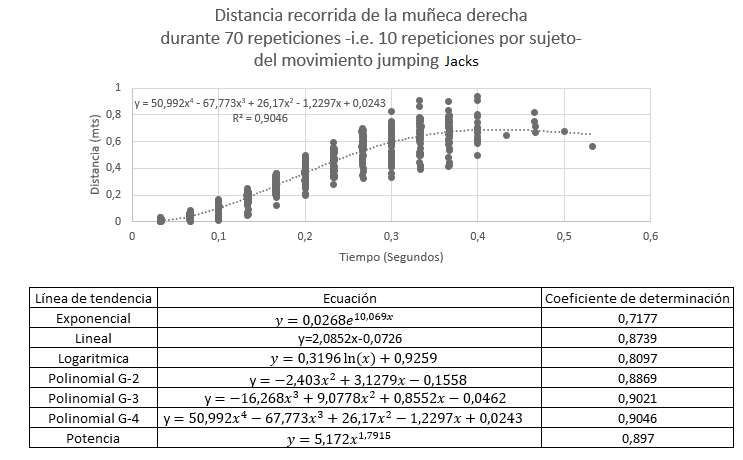
\includegraphics[width=445px,height=200px]{graphics/resultados/cluster-cheerleaders.PNG} \\
	\textbf{Fuente:} Recuperado por los v\'ideos etiquetados del trabajo de campo (ver secci\'on \ref{dis:even})
\end{figure}
\begin{figure}[H]
	\caption{Regresi\'on de muestra de tenis de mesa}
	\label{fig:regrTennisDeMesa}
	\centering
	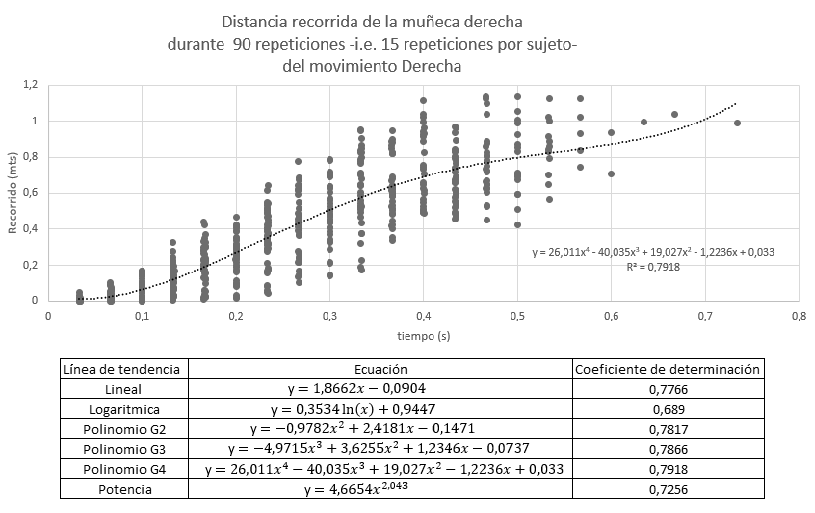
\includegraphics[width=445px,height=200px]{graphics/resultados/cluster-tennis.PNG} \\
	\textbf{Fuente:} Recuperado por los v\'ideos etiquetados del trabajo de campo (ver secci\'on \ref{dis:even})
\end{figure}